\documentclass{fkssolpub}

\usepackage[czech]{babel}
\usepackage{fontspec}
\usepackage{fkssugar}
\usepackage{amsmath}
\usepackage{graphicx}

\newcommand{\dd}{\mathrm{d}}
\renewcommand{\angle}{\sphericalangle}

\author{Ondřej Sedláček}
\school{Gymnázium Oty Pavla} 
\series{4}
\problem{4} 

\begin{document}




Celý tento důkaz směřujeme k důkazu, že průsečík kružnic ze zadání je ortocentrum $H$ trojúhelníku vyznačené středními příčkami trojúhelníku $ABC$. Pokud totiž toto platí, pak tento bod leží na Eulerově přímce, stejně jako střed kružnice opsané $S_aS_bS_c$ těžiště, které je pro trojúhelníky $ABC$ a $S_aS_bS_c$ stejné.

Jako první ukážeme, že kružnice opsané trojúhelníkům $AS_bS_c$, $BS_aS_c$ a $CS_aS_b$ se vždy po dvojicích protínají ve dvou bodech. Protože všechny tyto trojúhelníky jsou si shodné, pokud by se jedna dvojice kružnic protínala v jednom bodě, musí tyto trojúhelníky být pravoúhlé, protože jedna z jejich stran bude průměrem kružnice opsané (viz obr \ref{fig:right}). Tento příklad ale rozebíráme jen pro ostroúhlé trojúhelníky, tedy každá dvojice kružnic opsaných musí mít právě dva průsečíky.

Teď dokážeme, že průnik těchto kružnic je opravdu jediný bod. Nechť kružnice opsané trojúhelníkům $AS_bS_c$, $BS_aS_c$ se protínají kromě bodu $S_c$ v bodě $H$. Přes tětivové čtyřúhelníky zjistíme, že $|\angle S_aHS_b| = 360^{\circ} - |\angle S_aHS_c| - |\angle S_bHS_c| = 360^{\circ} - (180^{\circ} - \alpha) - (180^{\circ} - \beta) = \alpha + \beta = 180^{\circ} - \gamma$. Díky tomu z obvodových a středových úhlů víme, že bod $H$ leží i na kružnici opsané trojúhelníku $CS_aS_b$ a tedy se tyto kružnice opravdu protínají v jednom bodě.

Teď nám zbývá dokázat, že průsečík těchto kružnic je opravdu ortocentrum trojúhelníku $S_aS_bS_c$. K tomu dokážeme, že každá přímka $HS_a$, $HS_b$, $HS_c$ je výška v daném trojúhelníku. To ukáži důkazem, který je pro každou z přímek symetrický.

Nechť to tedy dokážeme pro přímku $HS_c$. Víme, že trojúhelník $AS_bS_c$ lze zobrazit na trojúhelník $BS_aS_c$ posunutím o vektor $\vect{AS_c}$. Z toho plyne, že spojnice středů těchto kružnic opsaných je rovnoběžná se stranou $AB$ a $S_aS_b$. A protože je přímka $HS_c$ chordálou těchto kružnic opsaných, je tato přímka kolmá na $S_aS_b$, což jsme chtěli ukázat.

Když tento postup zopakujeme pro všechny strany, dostaneme, že v průsečíku kružnic se protínají všechny výšky a tedy se jedná o ortocentrum trojúhelníku $S_aS_bS_c$. To jsme přesně chtěli dokázat, protože díky tomu tento bod leží na Eulerově přímce stejně jako střed kružnice opsané a těžnice. Q. E. D.


\begin{figure}[h!]
  \begin{center}
    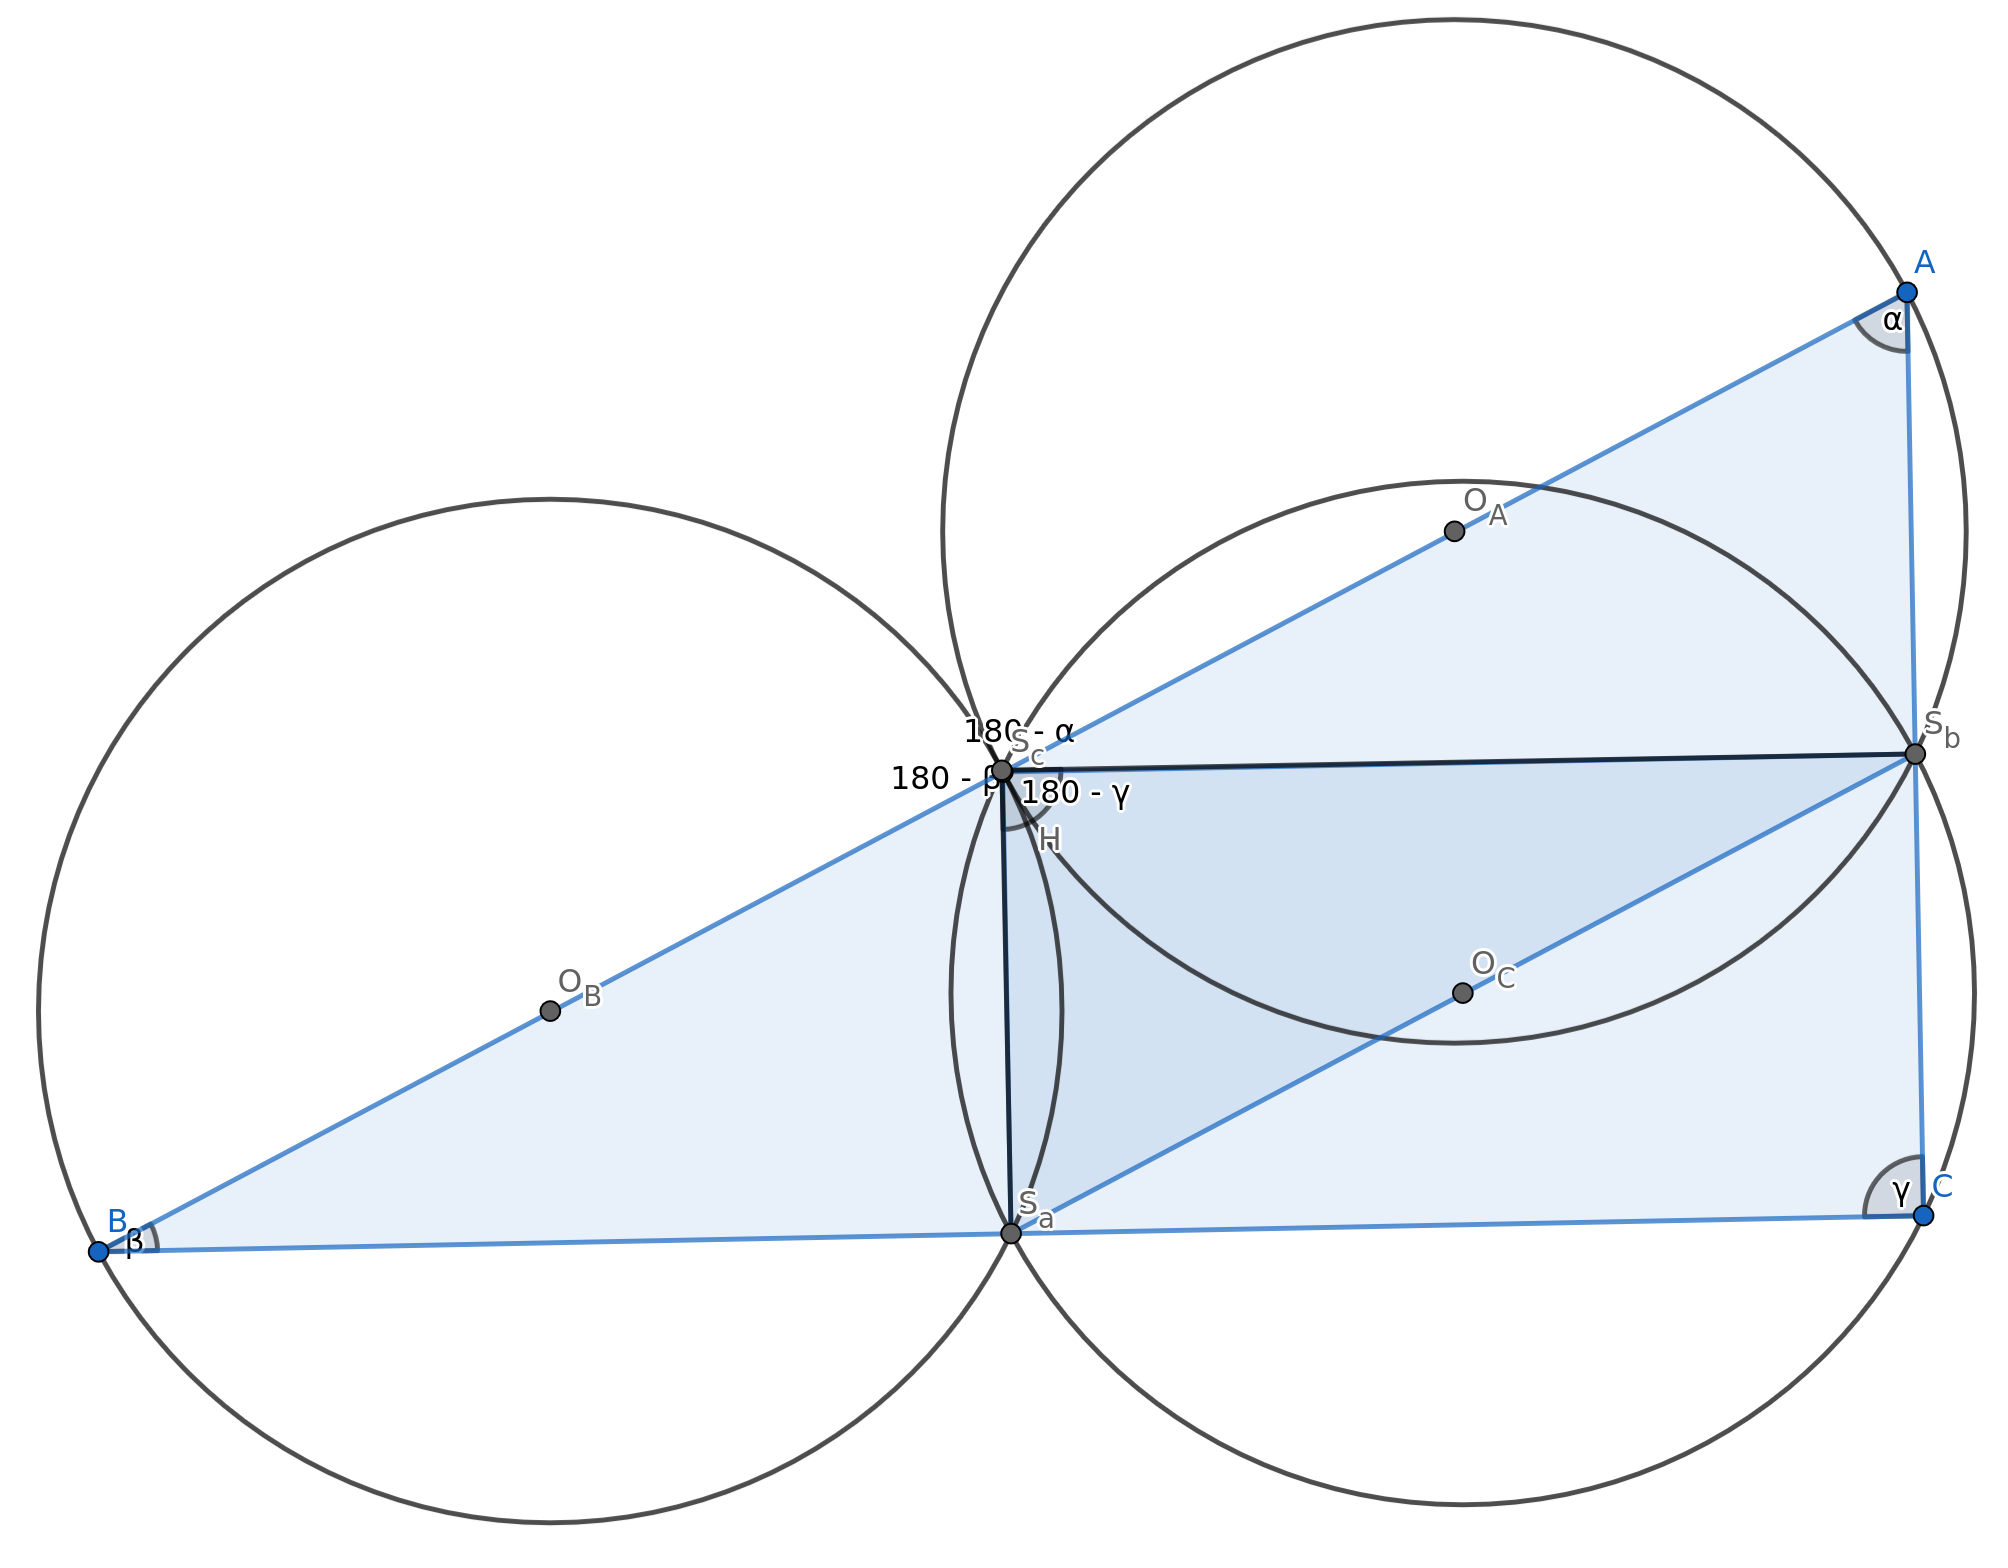
\includegraphics[width=0.65\textwidth]{4-1.png}
  \end{center}
  \caption{Případ pravoúhlého trojúhelníku}\label{fig:right}
\end{figure}

\begin{figure}[h!]
  \begin{center}
    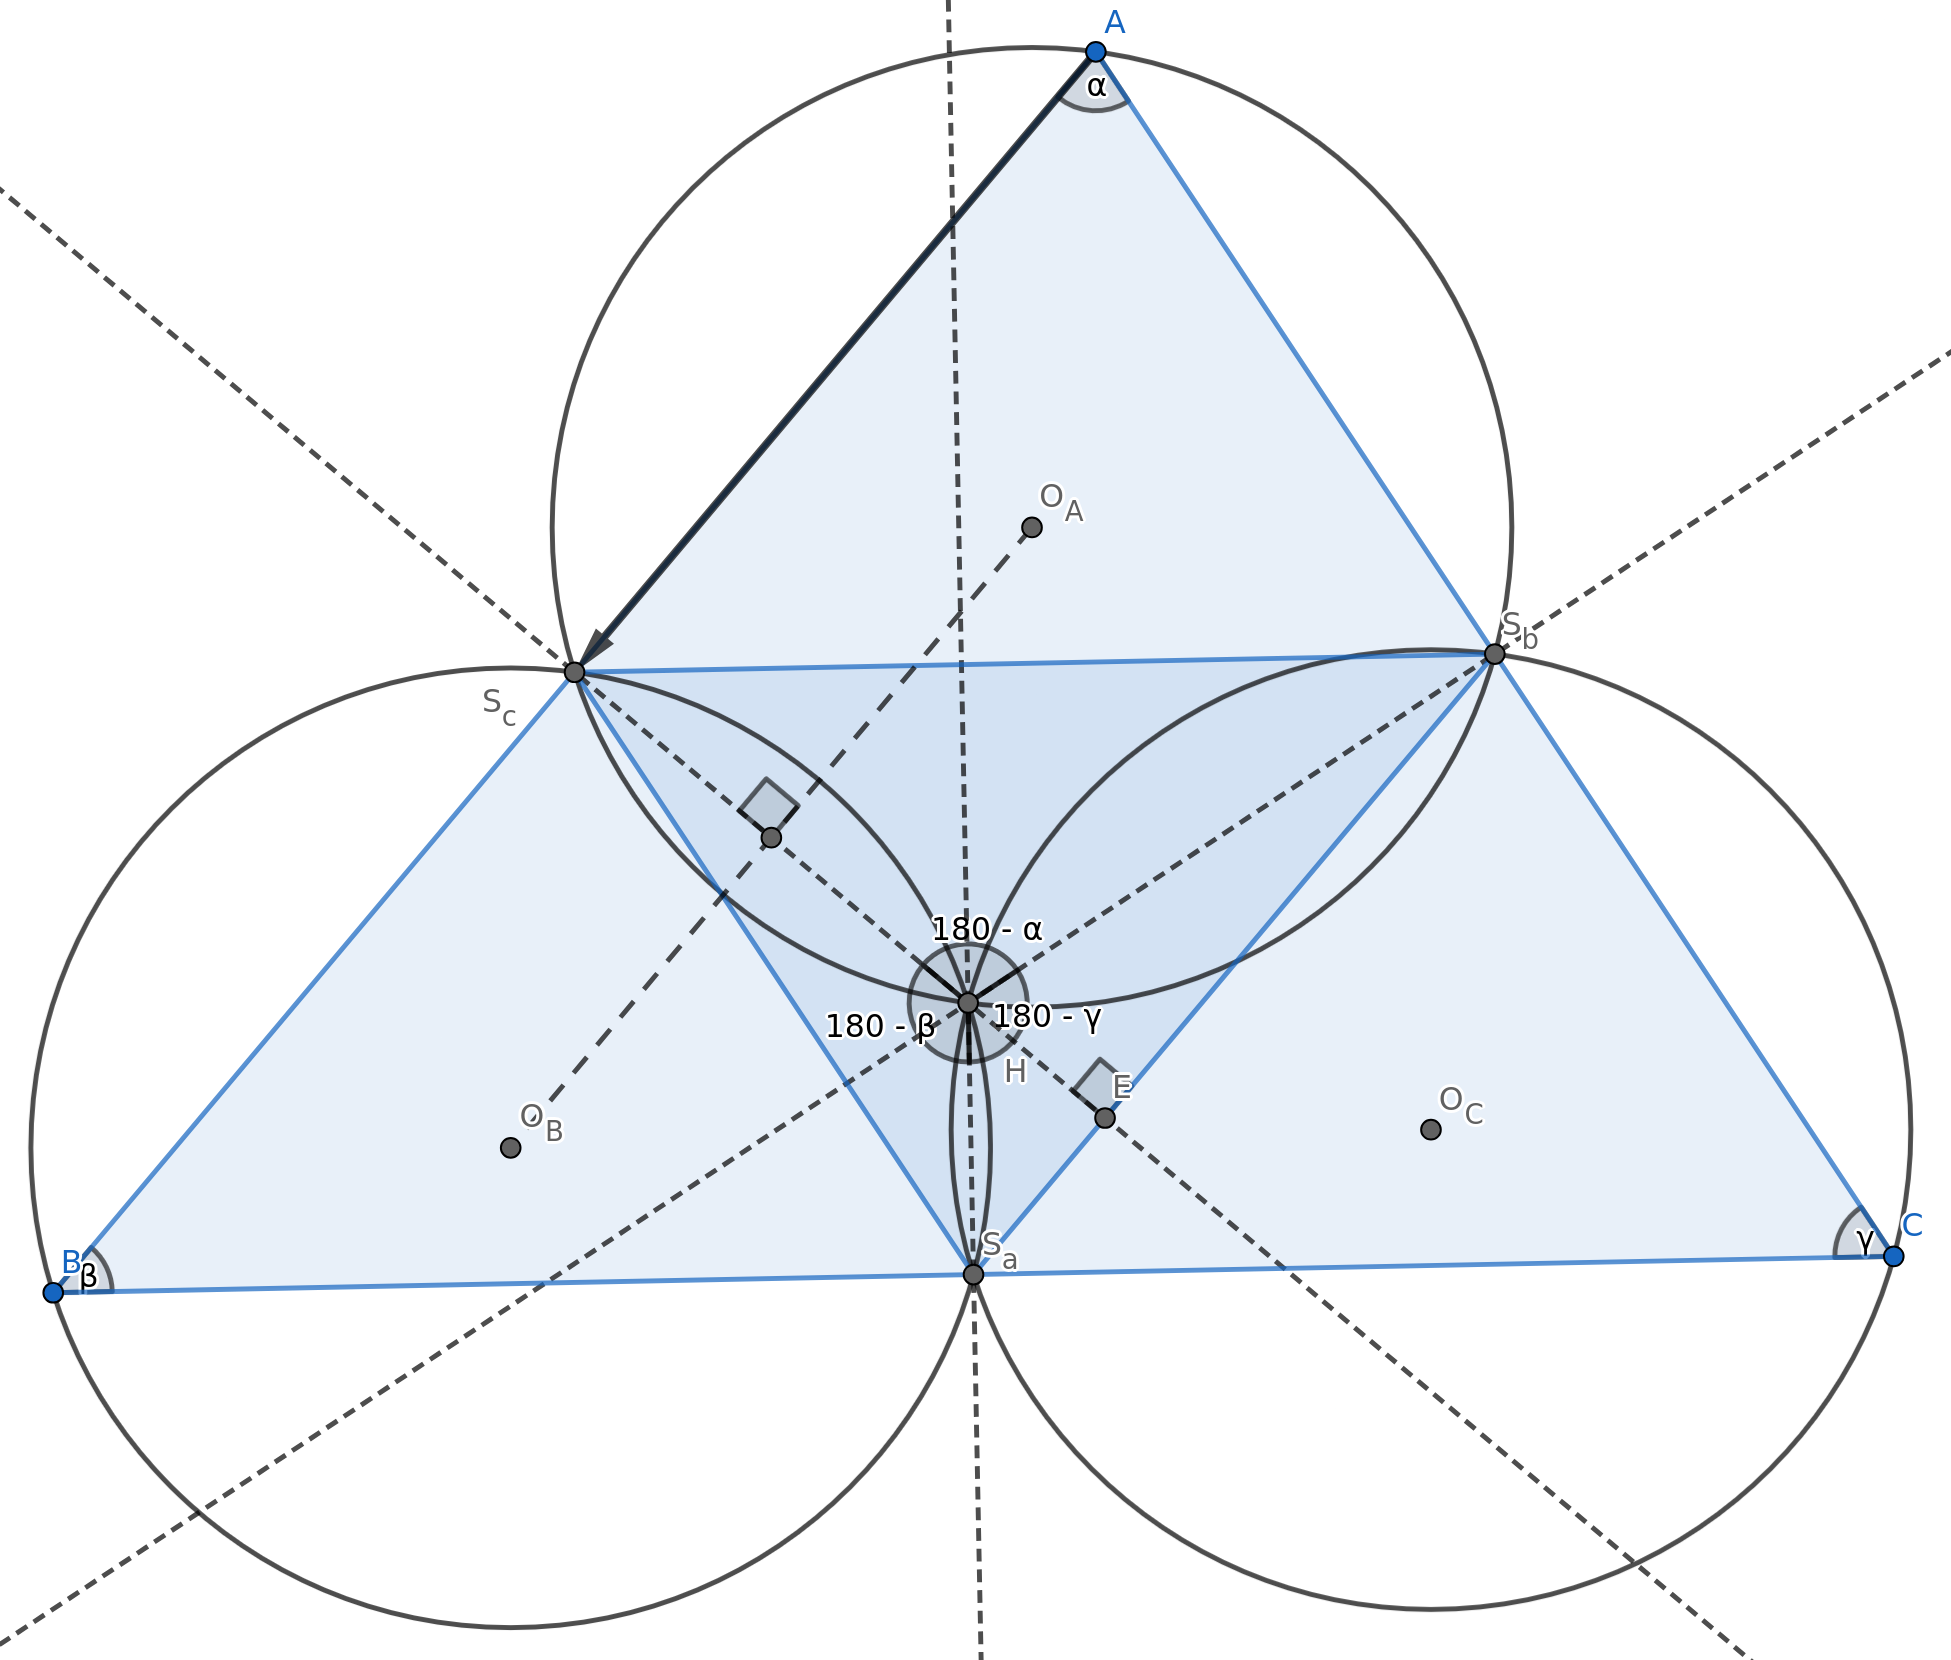
\includegraphics[width=0.95\textwidth]{4-2.png}
  \end{center}
  \caption{Pro důkaz, že se jedná o ortocentrum}\label{fig:2}
\end{figure}

\end{document}
